\chapter{Experimental Design\label{cha:chapter3}}

This chapter presents the methodology and experimental framework used to evaluate prompt framing sensitivity.

\section{Research Questions\label{sec:research-questions}}

In this study, we investigate four central research questions:

\begin{itemize}
\tightlist
\item
 \textbf{RQ1}: How large are prompt-framing effects relative to model effects for code-generation and math-reasoning tasks?
\item
 \textbf{RQ2}: Do tone, role framing, and prompt-wrapper format affect correctness, and are effects consistent across task kinds and model families?
\item
 \textbf{RQ3}: How do prompt factors affect observable behavior such as completion tokens, duration, result-only compliance, empty responses, and extraction failures?
\item
 \textbf{RQ4}: To what extent are correctness effects explained by behavioral variables such as verbosity, result-only compliance, and duration?
\end{itemize}

\section{Factorial Prompt Design\label{sec:factorial-prompt-design}}

This thesis adopts a 3 $\times$ 2 $\times$ 3 factorial design with three tones (neutral, polite, aggressive), two role-framing levels (no role, expert/developer role), and three prompt formats (plain text, JSON, XML), creating 18 prompt variants for each base task. The prompt framing factors and levels are summarized in Table~\ref{tab:prompt-factors}.

\begin{longtable}[]{@{}
 >{\raggedright\arraybackslash}p{(\linewidth - 4\tabcolsep) * \real{0.3333}}
 >{\raggedright\arraybackslash}p{(\linewidth - 4\tabcolsep) * \real{0.3333}}
 >{\raggedright\arraybackslash}p{(\linewidth - 4\tabcolsep) * \real{0.3333}}@{}}
\caption{Prompt framing factors and levels.}\label{tab:prompt-factors}\tabularnewline
\toprule\noalign{}
\begin{minipage}[b]{\linewidth}\raggedright
Factor
\end{minipage} & \begin{minipage}[b]{\linewidth}\raggedright
Levels
\end{minipage} & \begin{minipage}[b]{\linewidth}\raggedright
Purpose
\end{minipage} \\
\midrule\noalign{}
\endfirsthead
\toprule\noalign{}
\begin{minipage}[b]{\linewidth}\raggedright
Factor
\end{minipage} & \begin{minipage}[b]{\linewidth}\raggedright
Levels
\end{minipage} & \begin{minipage}[b]{\linewidth}\raggedright
Purpose
\end{minipage} \\
\midrule\noalign{}
\endhead
\bottomrule\noalign{}
\endlastfoot
Tone & Neutral, Polite, Aggressive & Test social framing and pressure cues \\
Role Framing & No Role, Expert/Developer Role & Test role/domain framing \\
Wrapper Format & Plain Text, JSON, XML & Test structured prompt wrapping \\
\end{longtable}

Task content remains the same across variants, only framing changes. The \texttt{Format} column in the prompt matrix determines how the task is formatted (plaintext, JSON, XML). It is therefore a prompt format, not a guaranteed structured output. Full prompt templates are treated as replication documentation, rather than being fully posted in the main content.

Below is a compact prompt skeleton to illustrate the intervention. Within each task kind, the same base problem text is inserted into the \texttt{task} slot for each of 18 variants. The variable cells change the instruction phrasing via tone and role framing, and also change whether the same instruction/task pair is represented as plaintext, JSON, or XML. Output-only constraints for the API runs are applied separately via system prompts, not as fields in the prompt matrix.

\begin{Shaded}
\begin{Highlighting}[]
Plaintext:
\{role/background sentence\}
\{neutral, polite, or aggressive task instruction\}
Task: \{PYTHON\_PROBLEM or MATH\_PROBLEM\}

JSON:
\{
 "instruction": "\{role/background sentence + task instruction\}",
 "task": "\{PYTHON\_PROBLEM or MATH\_PROBLEM\}"
\}

XML:
\textless{}prompt\textgreater{}
 \textless{}instruction\textgreater{}\{role/background sentence + task instruction\}\textless{}/instruction\textgreater{}
 \textless{}task\textgreater{}\{PYTHON\_PROBLEM or MATH\_PROBLEM\}\textless{}/task\textgreater{}
\textless{}/prompt\textgreater{}
\end{Highlighting}
\end{Shaded}

The experimental factors were intentionally designed to reflect normal user behavior rather than adversarial attacks. The polite prompts use grateful wording, the aggressive prompts apply pressure, the role prompts assign realistic personas, and the structured prompts wrap the task in JSON or XML. Consequently, the current research uses standard prompt engineering methods rather than red-team perturbation methods. Since every baseline task occurs in all variants, each attribute comparison evaluates output for the same underlying task distribution.

The crossed design also helps address an issue inherent to prompt comparison experiments: concurrently altering multiple factors. In manual prompt tuning, developers frequently change tone, amount of detail, prompt length, and format simultaneously. While such a prompt may lead to practical results, it is difficult to determine which component of the prompt was responsible for the effect. By separating tone, roles, and the wrapper format, our approach enables measuring each of the elements against a stable baseline while preserving realistic prompts.

Figure~\ref{fig:experimental_pipeline} summarizes the end-to-end experimental pipeline from task sources through prompt construction, model execution, extraction, evaluation, and analysis.

\begin{figure}[htbp]
\centering
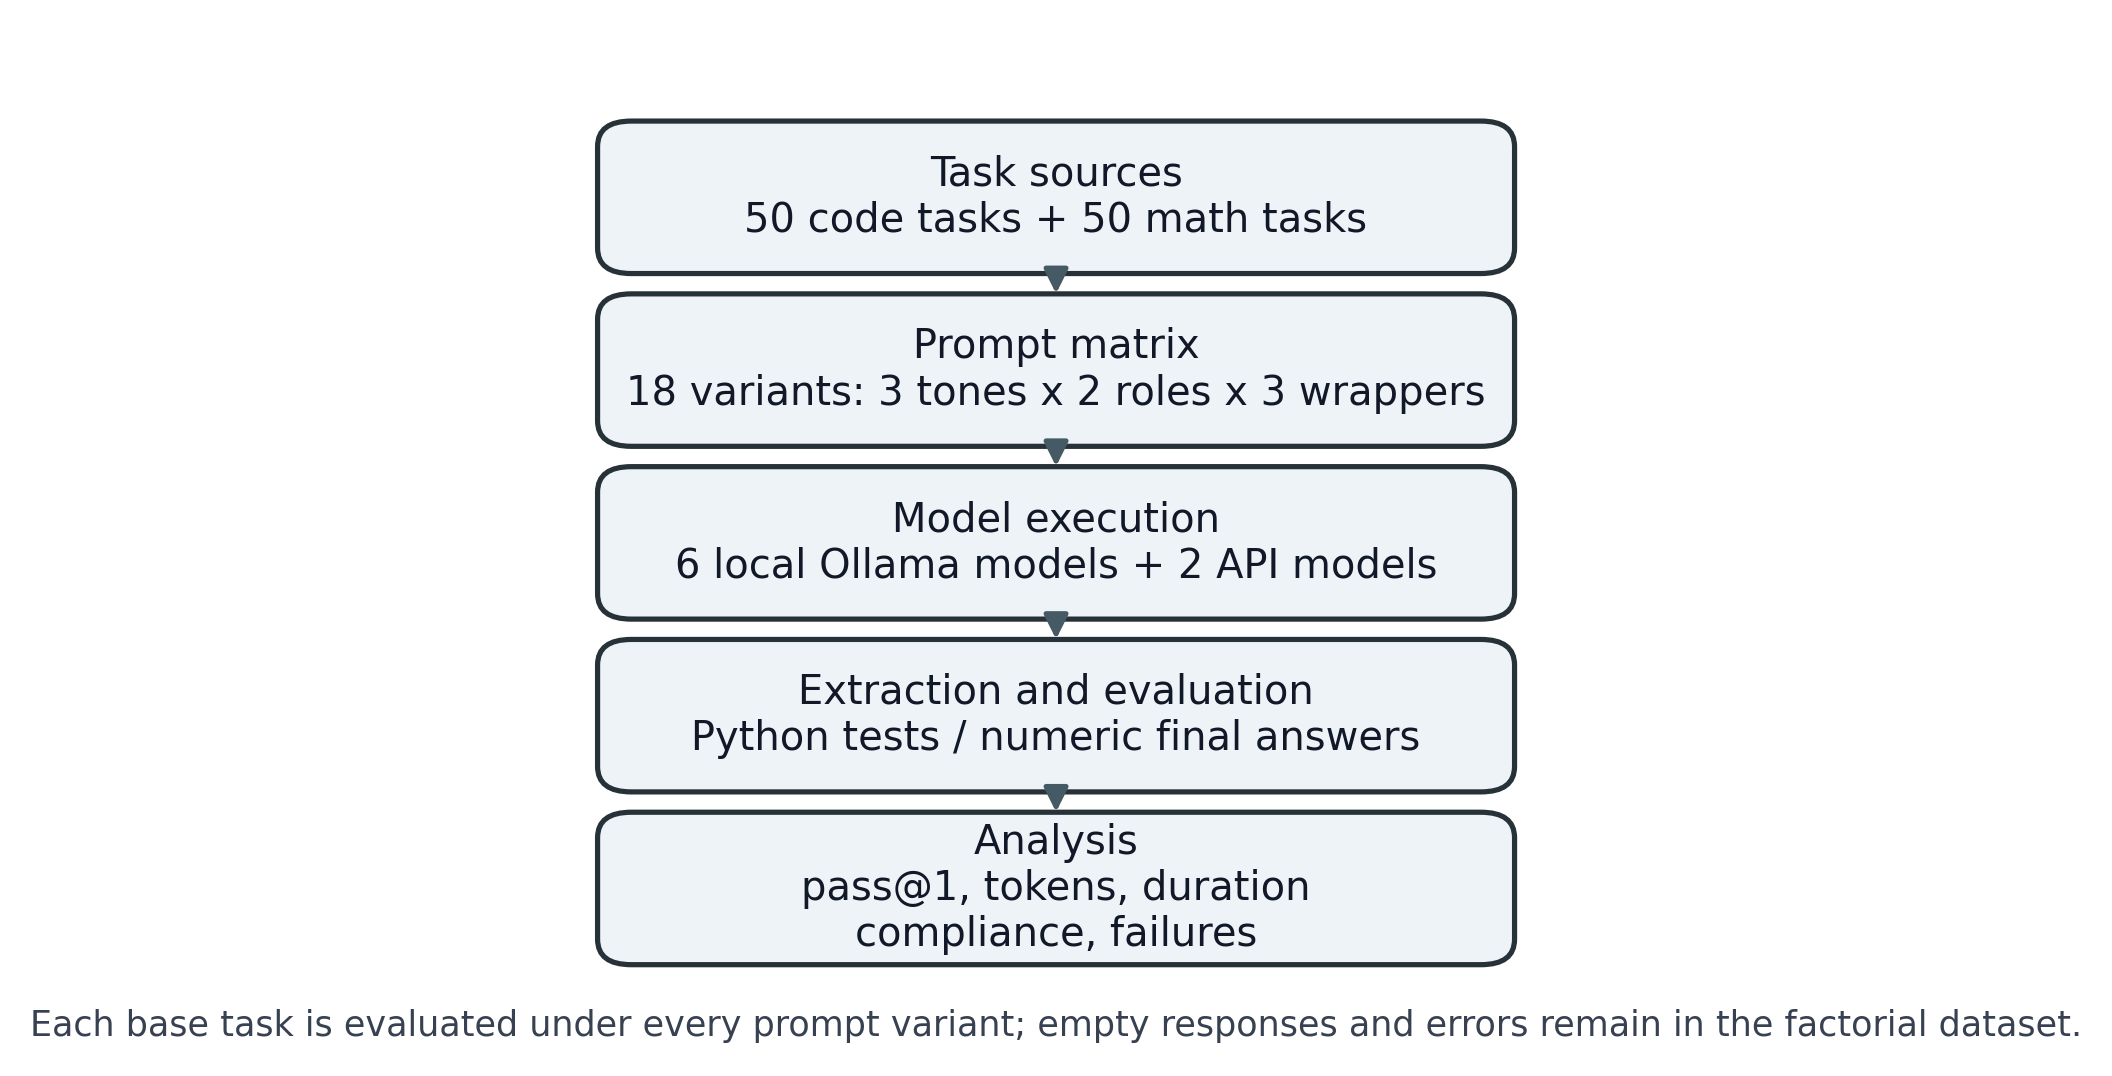
\includegraphics[width=0.95\linewidth,height=\textheight,keepaspectratio,alt={Experimental pipeline from task sources through the prompt matrix, model execution, extraction/evaluation, and analysis.}]{figures/experimental_pipeline.png}
\caption{Experimental pipeline from task sources through the prompt matrix, model execution, extraction/evaluation, and analysis.}
\label{fig:experimental_pipeline}
\end{figure}

\section{Models Evaluated\label{sec:models}}

The experiment includes two model groups: local models and cloud models (or API models). The six Ollama-hosted local models and their specifications are detailed in Table~\ref{tab:local-models}:

\begin{longtable}[]{@{}lrr@{}}
\caption{Local Ollama models evaluated in the experiment.}\label{tab:local-models}\tabularnewline
\toprule\noalign{}
Model & Parameters & Ollama package size \\
\midrule\noalign{}
\endfirsthead
\toprule\noalign{}
Model & Parameters & Ollama package size \\
\midrule\noalign{}
\endhead
\bottomrule\noalign{}
\endlastfoot
nemotron-3-nano-4b & 3.97B & 2.64 GiB \\
deepseek-coder-6.7b & 6.74B & 3.57 GiB \\
qwen2.5-7b & 7.0B & 4.36 GiB \\
mistral-7b-instruct & 7.24B & 4.07 GiB \\
llama3.1-8b & 8.0B & 4.58 GiB \\
gemma2-9b & 9.0B & 5.07 GiB \\
\end{longtable}

The local package sizes are quantized Ollama package sizes, not FP16 memory requirements. Quantized local deployment on consumer hardware is enabled by memory-efficient inference techniques \cite{alizadeh2023llmflash}. Model identifiers and public model-card information are used for the local model descriptions where available \cite{nemotron3nano2026, deepseekcoder2023, qwen25release2024, mistral7b2023, llama31modelcard2024, gemma2release2024}.

The cloud API models evaluated in this experiment are listed in Table~\ref{tab:api-models}:

\begin{longtable}[]{@{}ll@{}}
\caption{Cloud API models evaluated in the experiment.}\label{tab:api-models}\tabularnewline
\toprule\noalign{}
Reporting label & API model identifier \\
\midrule\noalign{}
\endfirsthead
\toprule\noalign{}
Reporting label & API model identifier \\
\midrule\noalign{}
\endhead
\bottomrule\noalign{}
\endlastfoot
Gemini Flash & \texttt{gemini-3.1-flash-lite-preview} \\
DeepSeek V4 Flash & \texttt{deepseek-ai/DeepSeek-V4-Flash} \\
\end{longtable}

Local and API models are reported separately because they differ in deployment settings, latency, response style, training and post-training procedures, serving infrastructure, and overall capability. Because these differences are confounded with the deployment regime itself, performance gaps between the two groups cannot be attributed to model ability alone.

The models were selected intentionally heterogeneous. The six local models represent lightweight, open-source deployments that a practitioner could run through Ollama, while the two API models represent commercial systems with stronger infrastructure and different serving behavior. This split is not to rank all available LLMs or create a general benchmark. It is used to test whether the effects of prompt-factor patterns remain stable when moving between different local and cloud settings. As the results show, stability cannot be assumed.

Separating local and API results also protects the validity of latency and output behavior. Local runtimes are governed by local inference stacks and quantized weights, whereas API runtimes are influenced by hosted serving infrastructure and network conditions. Combining them into a single timing metric would be misleading. Therefore, this thesis treats local and API findings as distinct but complementary evidence of how prompt sensitivity reacts to different deployment regimes.

\section{Tasks and Datasets\label{sec:tasks}}

The study evaluates two task types: Python code generation and final-answer mathematical reasoning. Code generation acts as the primary software-engineering benchmark, requiring models to produce functional Python code to meet specific requirements. An automated evaluation pipeline then extracts the generated code and executes it against test cases. Mathematical tasks function as a secondary validation domain, where the evaluator isolates the model's final answer and compares it against the expected result.

Local and API models were evaluated on different problem sets. Local code tasks are derived from high-school graduation and mock-exam math problems from the ToanMath THPT archive and converted into executable Python code \cite{toanmath2026thpt, promptframingkaggle2026}, while local math tasks use single-answer numeric problems filtered from VietJack's 2026 grade-10 entrance exam archive \cite{vietjack2026onvao10, promptframingkaggle2026}. API models use a paired MathNet-derived competition-math set with 50 problems for math and their Python conversions for code \cite{promptframingkaggle2026}. Because the models, task datasets, serving environments, and execution settings all differ between the two groups, the local and API experiments are designed as complementary experiments under different settings, not as head-to-head comparisons on a shared problem source; throughout this thesis, differences between the two groups are interpreted as differences between experimental settings rather than as model-ability rankings.

For every combination of model and task type, 50 base tasks are evaluated across 18 prompt variations, producing 900 individual runs per model--task kind. In total, the experiment encompasses 14,400 runs, 10,800 from local models and 3,600 from API models. The total run counts broken down by model group and task kind are presented in Table~\ref{tab:run-counts}.

The task sets are intentionally created with an equal number of prompts and levels of difficulty; otherwise, the comparison could create the false impression that one prompt type is better than the other on easier tasks. The research design guarantees that the framing effect can be examined for each task without reflecting only the problem-related content.

Both domains serve different functions. Software development is the first domain, as it is centered around code generation that produces usable products. Math problems are used for validation. The problems in this domain require multiple derivations but only produce a short answer that can be judged as objectively correct. Therefore, the combination of the two domains allows us to determine whether the prompt framing strategies that enhance code generation will have a similar effect on the final answer to a math problem.

Because coding challenges involve converting mathematical problems into Python, their representativeness for software-engineering code generation requires explicit discussion. This controlled task design was chosen deliberately for three reasons. First, math-derived problems have definitive, automatically checkable answers and test suites, allowing pass/fail scoring without human judgment across all 14,400 runs. Second, the short, self-contained nature of these problems keeps task difficulty constant while only the prompt framing changes, which is necessary to isolate tone, role, and format effects in a factorial design. Third, a single-attempt protocol on compact tasks ensures uniformity across the evaluation pipeline, including extraction, execution, and test harnesses. What this design primarily measures is controlled initial code generation: how prompt framing affects a model's first, single-shot attempt and its compatibility with an automated evaluator. However, it does not represent repository-level software development, such as multi-file context, iterative debugging, test-repair loops, code review, or long-horizon agent behavior. Therefore, the conclusions of this thesis should be interpreted as evidence regarding prompt framing in controlled initial code generation and final-answer reasoning, rather than as claims about LLM performance in realistic software projects.

\begin{longtable}[]{@{}lrrrr@{}}
\caption{Run counts by model group and task kind.}\label{tab:run-counts}\tabularnewline
\toprule\noalign{}
Group & Models & Task kinds & Runs per model-task kind & Total runs \\
\midrule\noalign{}
\endfirsthead
\toprule\noalign{}
Group & Models & Task kinds & Runs per model-task kind & Total runs \\
\midrule\noalign{}
\endhead
\bottomrule\noalign{}
\endlastfoot
Local models & 6 & 2 & 900 & 10,800 \\
API models & 2 & 2 & 900 & 3,600 \\
Total & 8 & 2 & - & 14,400 \\
\end{longtable}

\section{Execution Environment and Run Protocol\label{sec:execution-environment}}

We evaluate each prompt variant using a single-response approach, with pass@1 as the main metric. We keep the base task consistent across all variants, meaning that each variant is evaluated on every base task. Furthermore, to keep the factorial design fully intact, we retain blank outputs and errors rather than discarding them.

The local result files cover runs from 12 to 14 May 2026, logging Ollama model identifiers, timestamps, execution duration, prompt and completion token counts, generated responses, extracted code/numerical values, and evaluation results. Similarly, the API result files log runs conducted during the same period, detailing model identifiers and labels, timestamps, raw usage statistics, API response metadata, text, and evaluation results.

The evaluation framework uses an OpenAI-compatible chat-completions interface for its API runners. The default API settings in the runner are a temperature of 0, a maximum of 2048 generated tokens, a 120-second API timeout, a 10-second timeout for Python code execution, and a 2-second delay between requests. System prompts strictly instruct the model to "Output only the code, no explanations" for Python programming tasks and "Output only the final result, no explanations" for mathematical tasks. Furthermore, the system retains quota error logs and token-rotation metadata when utilizing multiple API keys, and holds execution states so it can resume running later if interrupted.

For local evaluations, the Ollama runners capture response times and token usage directly from Ollama's metadata. The specific configuration for the local math runner includes a temperature of 0, a 300-second request timeout, a 256-token generation limit, and a 0.2-second delay between calls. Legacy local code notebooks follow the same automated extraction and testing protocols, maintaining the 10-second execution timeout per test. Across all configurations, the top-p parameter is left at its default value for the respective provider or Ollama, meaning it is not treated as an experimental variable. Finally, the replication package includes comprehensive documentation: sanitized API configurations, details on the local Ollama setup, notebook environment specifications, and the retry and error-handling mechanisms applied to the six local models.

The system prompts have been made intentionally strict to enable automated evaluation and reduce ambiguity of results. However, it should be emphasized that automated evaluation still requires compliance measurement. Models may nevertheless provide additional explanatory text, ignore the required output format, generate no output at all, or produce unexpected formats. Although there is no need to get rid of all such examples, it is crucial that they demonstrate how the prompt policy works in practical applications as opposed to being just experimental noise.

The single-response approach is very important for interpretation purposes. It keeps the above calculations valid and prohibits iterative fixing of the generated responses. Actual agents use feedback to correct their mistakes; however, it should be noted that if revisions are allowed, it will not be easy to extract the effect of the prompt framing. Evaluating the model against only one attempt allows separating the effect of the manipulated prompt parameters on the model-evaluator pair.

\section{Outcome Measures\label{sec:outcome-measures}}

The experiment results are presented in the form of pass@1. For coding tasks, for a task to be considered passed, the produced Python code must pass all tests, including two examples provided in the prompts and five hidden tests. For mathematics problems, the solution passes if the extracted answer is the same as the required one after normalization.

Secondary outcomes describe observable behavior, including instruction-following-style compliance with the expected output form \cite{zhou2023ifeval}:

\begin{itemize}
\tightlist
\item
 \textbf{Completion tokens}: number of generated tokens.
\item
 \textbf{Duration}: response latency in seconds.
\item
 \textbf{Result-only compliance}: whether the response is close to the expected compact output form.
\item
 \textbf{Code-only compliance}: whether code responses are mostly clean, executable code.
\item
 \textbf{Empty responses}: responses with no usable output.
\item
 \textbf{Extraction failures and error modes}: cases where the output cannot be parsed or evaluated.
\end{itemize}

These outcomes are central to this thesis because prompt design can affect a system's usefulness even without improving correctness.

We interpret these behavioral outcomes as engineering signals: completion tokens approximate cost and verbosity, duration estimates latency, and compliance approximates the ease with which downstream tools can consume the response. Furthermore, empty outputs and extraction failures expose brittle points in the evaluation pipeline. Rigorous execution-based evaluation of code LLMs shows that evaluator design choices---extraction rules, test harnesses, and normalization---are themselves a significant source of variation across runners \cite{liu2023nece}. The broader shift toward using LLMs as automated judges introduces additional considerations about evaluation reliability and bias \cite{li2025llmjudge}. Reporting these dimensions alongside pass@1 enables us to distinguish prompts that yield genuine accuracy gains from those that simply trade off accuracy for cost, cleanliness, speed, or parser compatibility.

Our definition of compliance is practical rather than philosophical. Result-only compliance does not show that the model understood the instruction, and code-only compliance does not show that the code is correct. Instead, the evaluation only considers whether the response fulfilled the formal requirements of the evaluation pipeline, since LLMs function as parts of larger integrated systems.
